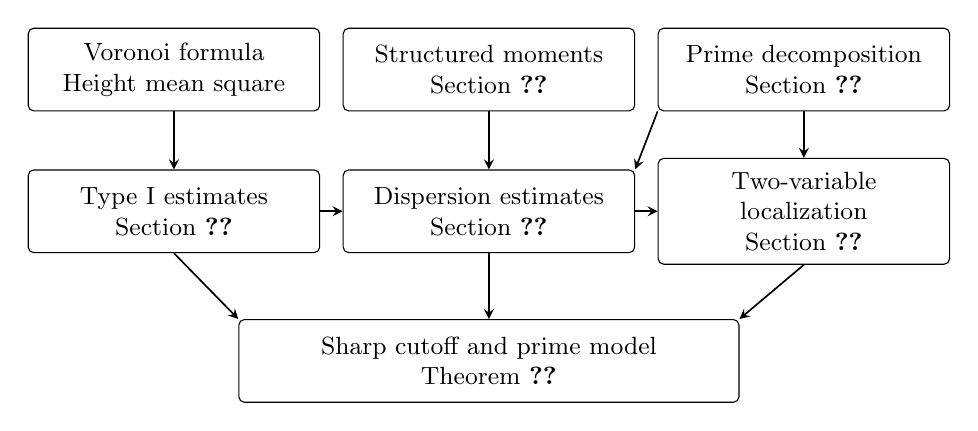
\begin{tikzpicture}[x=1cm,y=1cm,
 box/.style={draw,rounded corners=2pt,align=center,font=\small,
             text width=3.35cm,minimum height=1.05cm,inner sep=5pt},
 arrow/.style={->,>=stealth,semithick}]
\node[box] (level) at (-4,3.4) {Voronoi formula\\Height mean square};
\node[box] (moments) at (0,3.4) {Structured moments\\Section~\ref{sec:dual}};
\node[box] (decomp) at (4,3.4) {Prime decomposition\\Section~\ref{sec:decomposition}};
\node[box] (typei) at (-4,1.6) {Type~I estimates\\Section~\ref{sec:typeI}};
\node[box] (low) at (0,1.6) {Dispersion estimates\\Section~\ref{sec:dispersion}};
\node[box] (high) at (4,1.6) {Two-variable localization\\Section~\ref{sec:perron}};
\node[box,text width=6cm] (end) at (0,-.3) {Sharp cutoff and prime model\\Theorem~\ref{thm:main}};
\draw[arrow] (level)--(typei);
\draw[arrow] (moments)--(low);
\draw[arrow] (typei)--(low);
\draw[arrow] (decomp)--(high);
\draw[arrow] (decomp.south west)--(low.north east);
\draw[arrow] (low)--(high);
\draw[arrow] (typei.south)--(end.north west);
\draw[arrow] (low)--(end);
\draw[arrow] (high.south)--(end.north east);
\end{tikzpicture}
